%!TEX root = ../hutbthesis_main.tex

\chapter{人机交互强化策略分析与系统优化}

\section{风险识别与告警分级策略}

固定翼飞行器着陆阶段的风险并非在接地瞬间才会出现，而是在进近、拉平、接地区域逐渐累积起来。所以人机交互强化首先需要解决的问题便是及时识别关键风险，再通过分级告警的方式去提醒操纵者。从前面的仿真结果能够知道，复杂地形、下沉率偏大、侧偏增加还有姿态波动加剧，这些都会提高着陆风险，特别是在山脊地形和阶跃地形当中，这种风险更为显著。

本文的观点是，风险识别应当围绕着飞行速度、下沉率、俯仰角、滚转角、侧偏量、航向误差、跑道相对位置等状态量来进行。其中，速度能够主要反映出是否存在失速或者过快接地的风险，下沉率主要反映的是接地冲击风险，俯仰角与滚转角主要反映姿态超限风险，侧偏量、航向误差反映的是跑道对准状态。为了提高提示的效果，本文把告警划分成了三级：一级是提示级，意思是状态偏离了目标但还没有接近边界，二级是警示级，意味着关键参数接近限制范围，三级是危险级，表明系统已经接近或者进入了明显不利窗口，在这个时候应该触发保护逻辑或者复飞/中止机制。吕健玮等人在无人机短距着陆控制技术研究里指出，短距着陆条件下控制窗口更小，所以风险识别必须提前进行。这一思路同样适用于本文的固定翼飞行器着陆控制系统。

\begin{figure}[H]
\centering
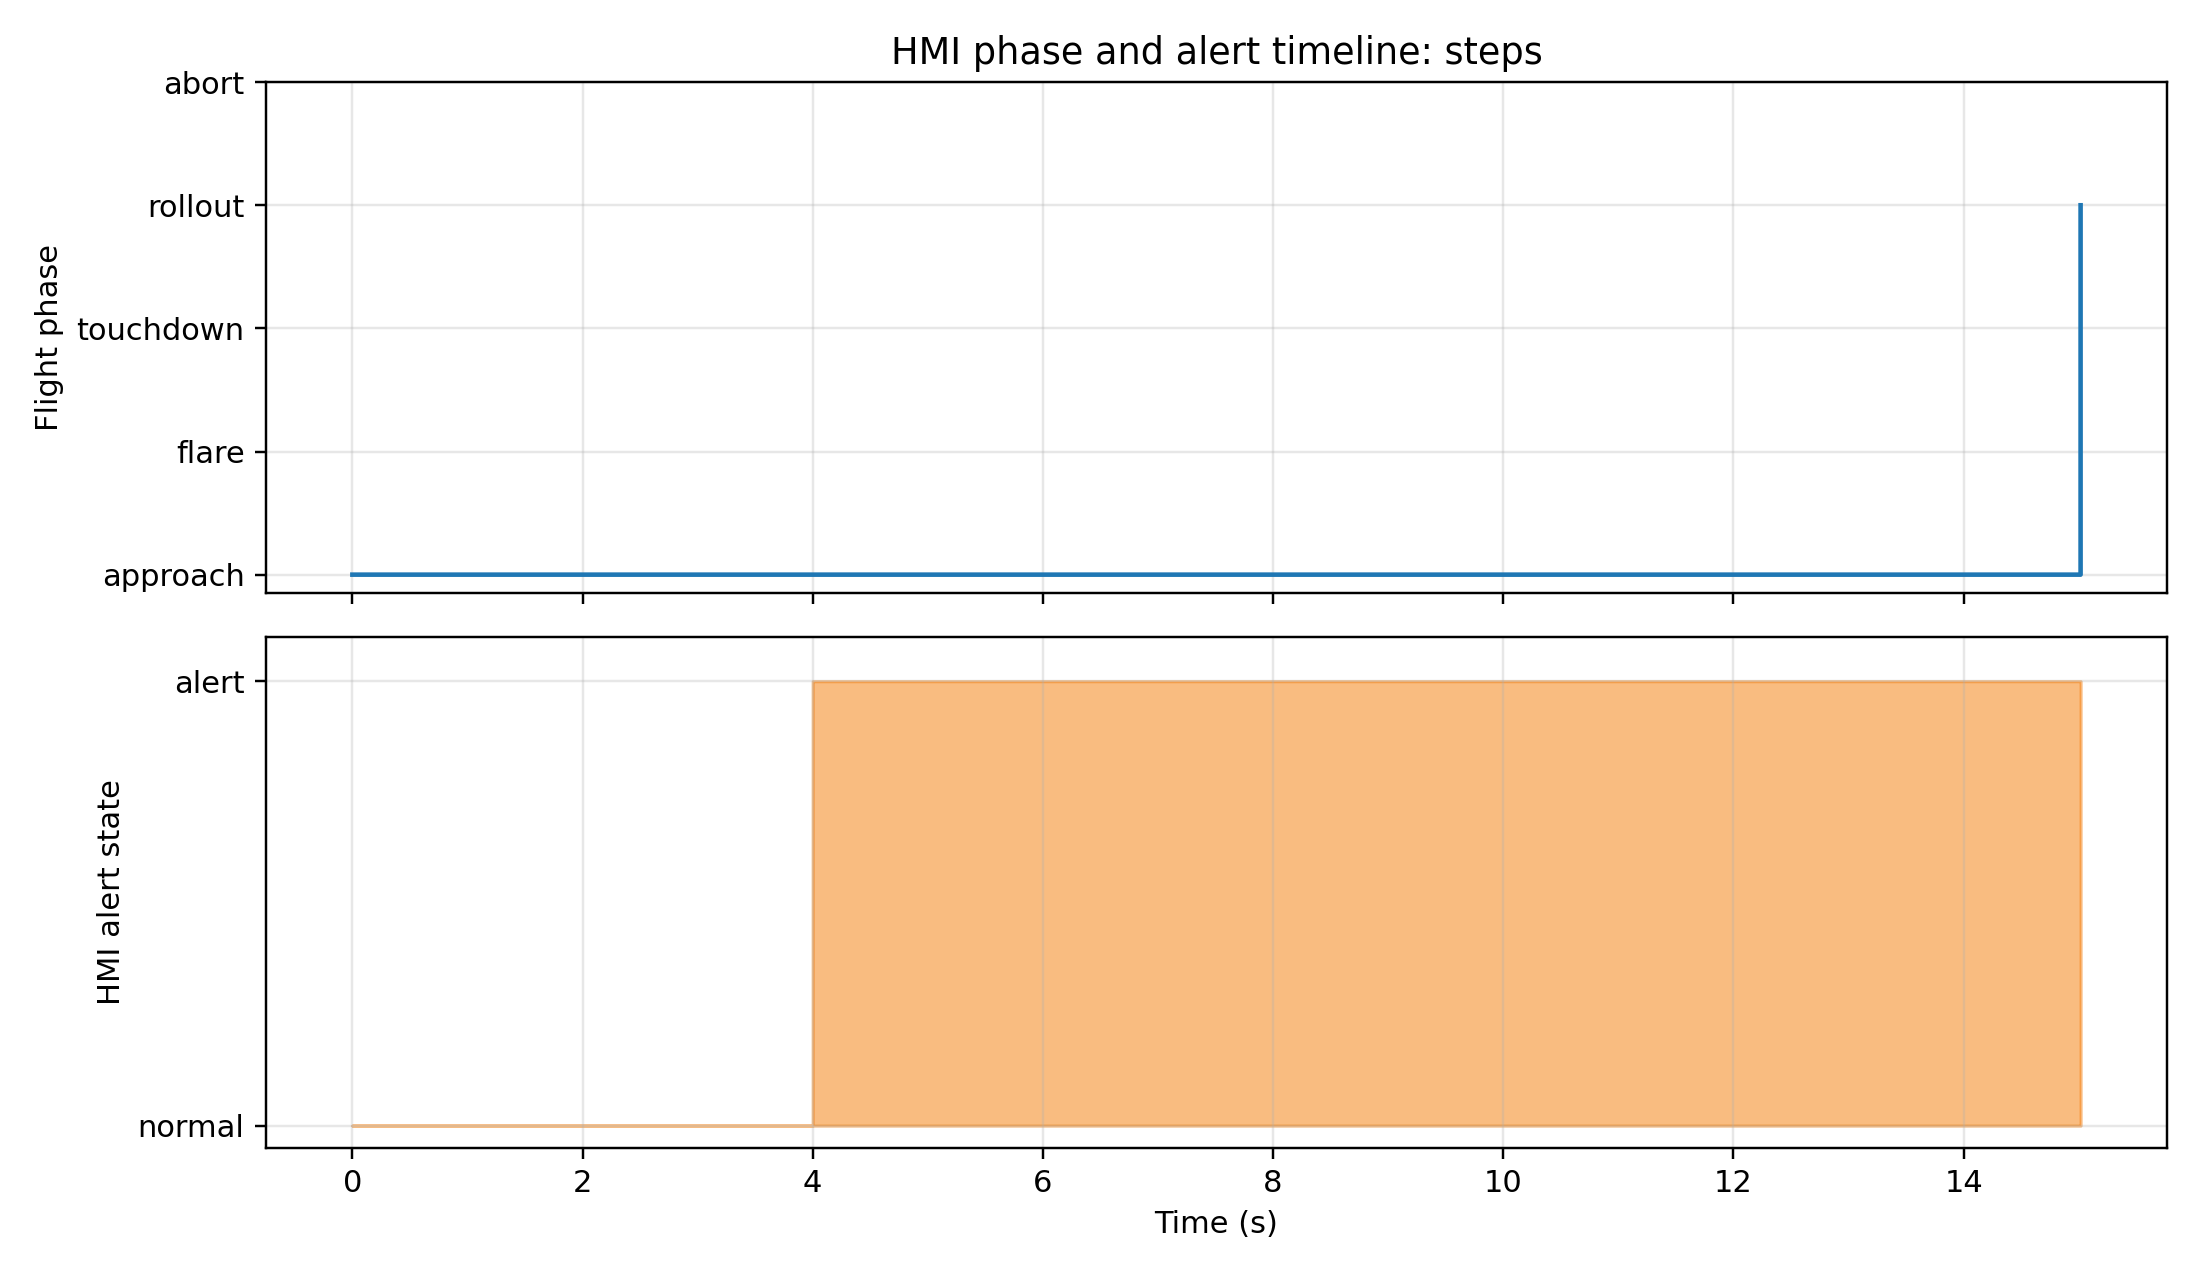
\includegraphics[width=0.92\linewidth,height=0.66\textheight,keepaspectratio]{images/image16.png}
\caption{阶跃地形工况下飞行阶段与HMI告警状态变化}
\label{fig:6-1}
\end{figure}

图~\ref{fig:6-1}以阶跃地形工况为例，展示了飞行阶段与HMI告警状态随进近过程的变化。可以看到，告警状态随进近、捕获和接地阶段动态变化，充分体现了HMI对风险状态的实时提示能力。

\section{状态提示、操纵辅助与约束控制设计}

在人机交互强化设计当中，风险识别仅仅只是基础内容，而真正对改善着陆品质起到关键作用的是状态提示、操纵辅助、约束控制这三者的协同配合。此篇论文依据现有的仿真平台界面、控制逻辑，把人机交互强化功能归纳为``提示---辅助---约束''这样的三层结构。第一层为状态提示层，第二层是操纵辅助层，第三层是约束控制层。这三层结构会按照由弱到强的顺序逐渐介入，如此既能保留操纵者的参与感，又能够在高风险阶段给予必要的保护。

状态提示层设计的关键在于追求``简单、直接、可理解''。因为着陆末段操纵负荷比较高，系统不应给操纵者传递过多冗余信息，而是要着重展示最关键的状态量。具体涵盖离地高度、速度、下沉率、俯仰角、滚转角、侧偏量、跑道剩余距离、目标接地点相对位置等。并且能够借助颜色变化、趋势箭头或者文字提示等形式，对``偏大''\,``偏小''\,``趋于危险''等状态予以直观呈现。例如，当下沉率不断增大时，给出``近地阶段下沉率偏大''的提示，当侧偏量迅速增大时，提示``检测到侧偏，正在修正''，当进入跑道捕获区时，提示``已进入跑道捕获区，优先保持接地稳定''。这种状态提示设计的作用，并非取代操纵者进行判断，而是减轻其在末段的信息整合负担。

操纵辅助层的关键要点是``给予方向，而非进行替代''。当飞行器状态快要接近风险边界，然而还未进入危险状态的时候，系统需要向操纵者输出相关建议信息，像是建议增大或者减小俯仰修正、提醒保持中心线、提示优先控制下沉率等情况。对于末段着陆来讲，这种辅助有着特别重要的意义，这是因为操纵者常常会在高度快速发生变化时出现操作方面的犹豫或者过度修正。段鹏在无人机短距着陆纵向控制技术研究里表明，短距着陆纵向控制的关键之处在于接地前速度和下沉率的协同约束。这一结论意味着，在人机交互强化的过程中，操纵辅助不应该是模棱两可的``注意安全''，而应该尽可能围绕纵向控制核心变量给出清晰明确的建议。

为验证不同控制模式的效果，本文在阶跃地形这一不利工况下，对比了正常模式与保守模式。从图~\ref{fig:6-2}可以看出，保守模式通过更高的速度安全裕度和襟翼约束，使接地阶段高度余量由正常模式的约1.20
ft提高到约4.68 ft，这体现了人机交互强化策略对风险工况的辅助作用。

\begin{figure}[H]
\centering
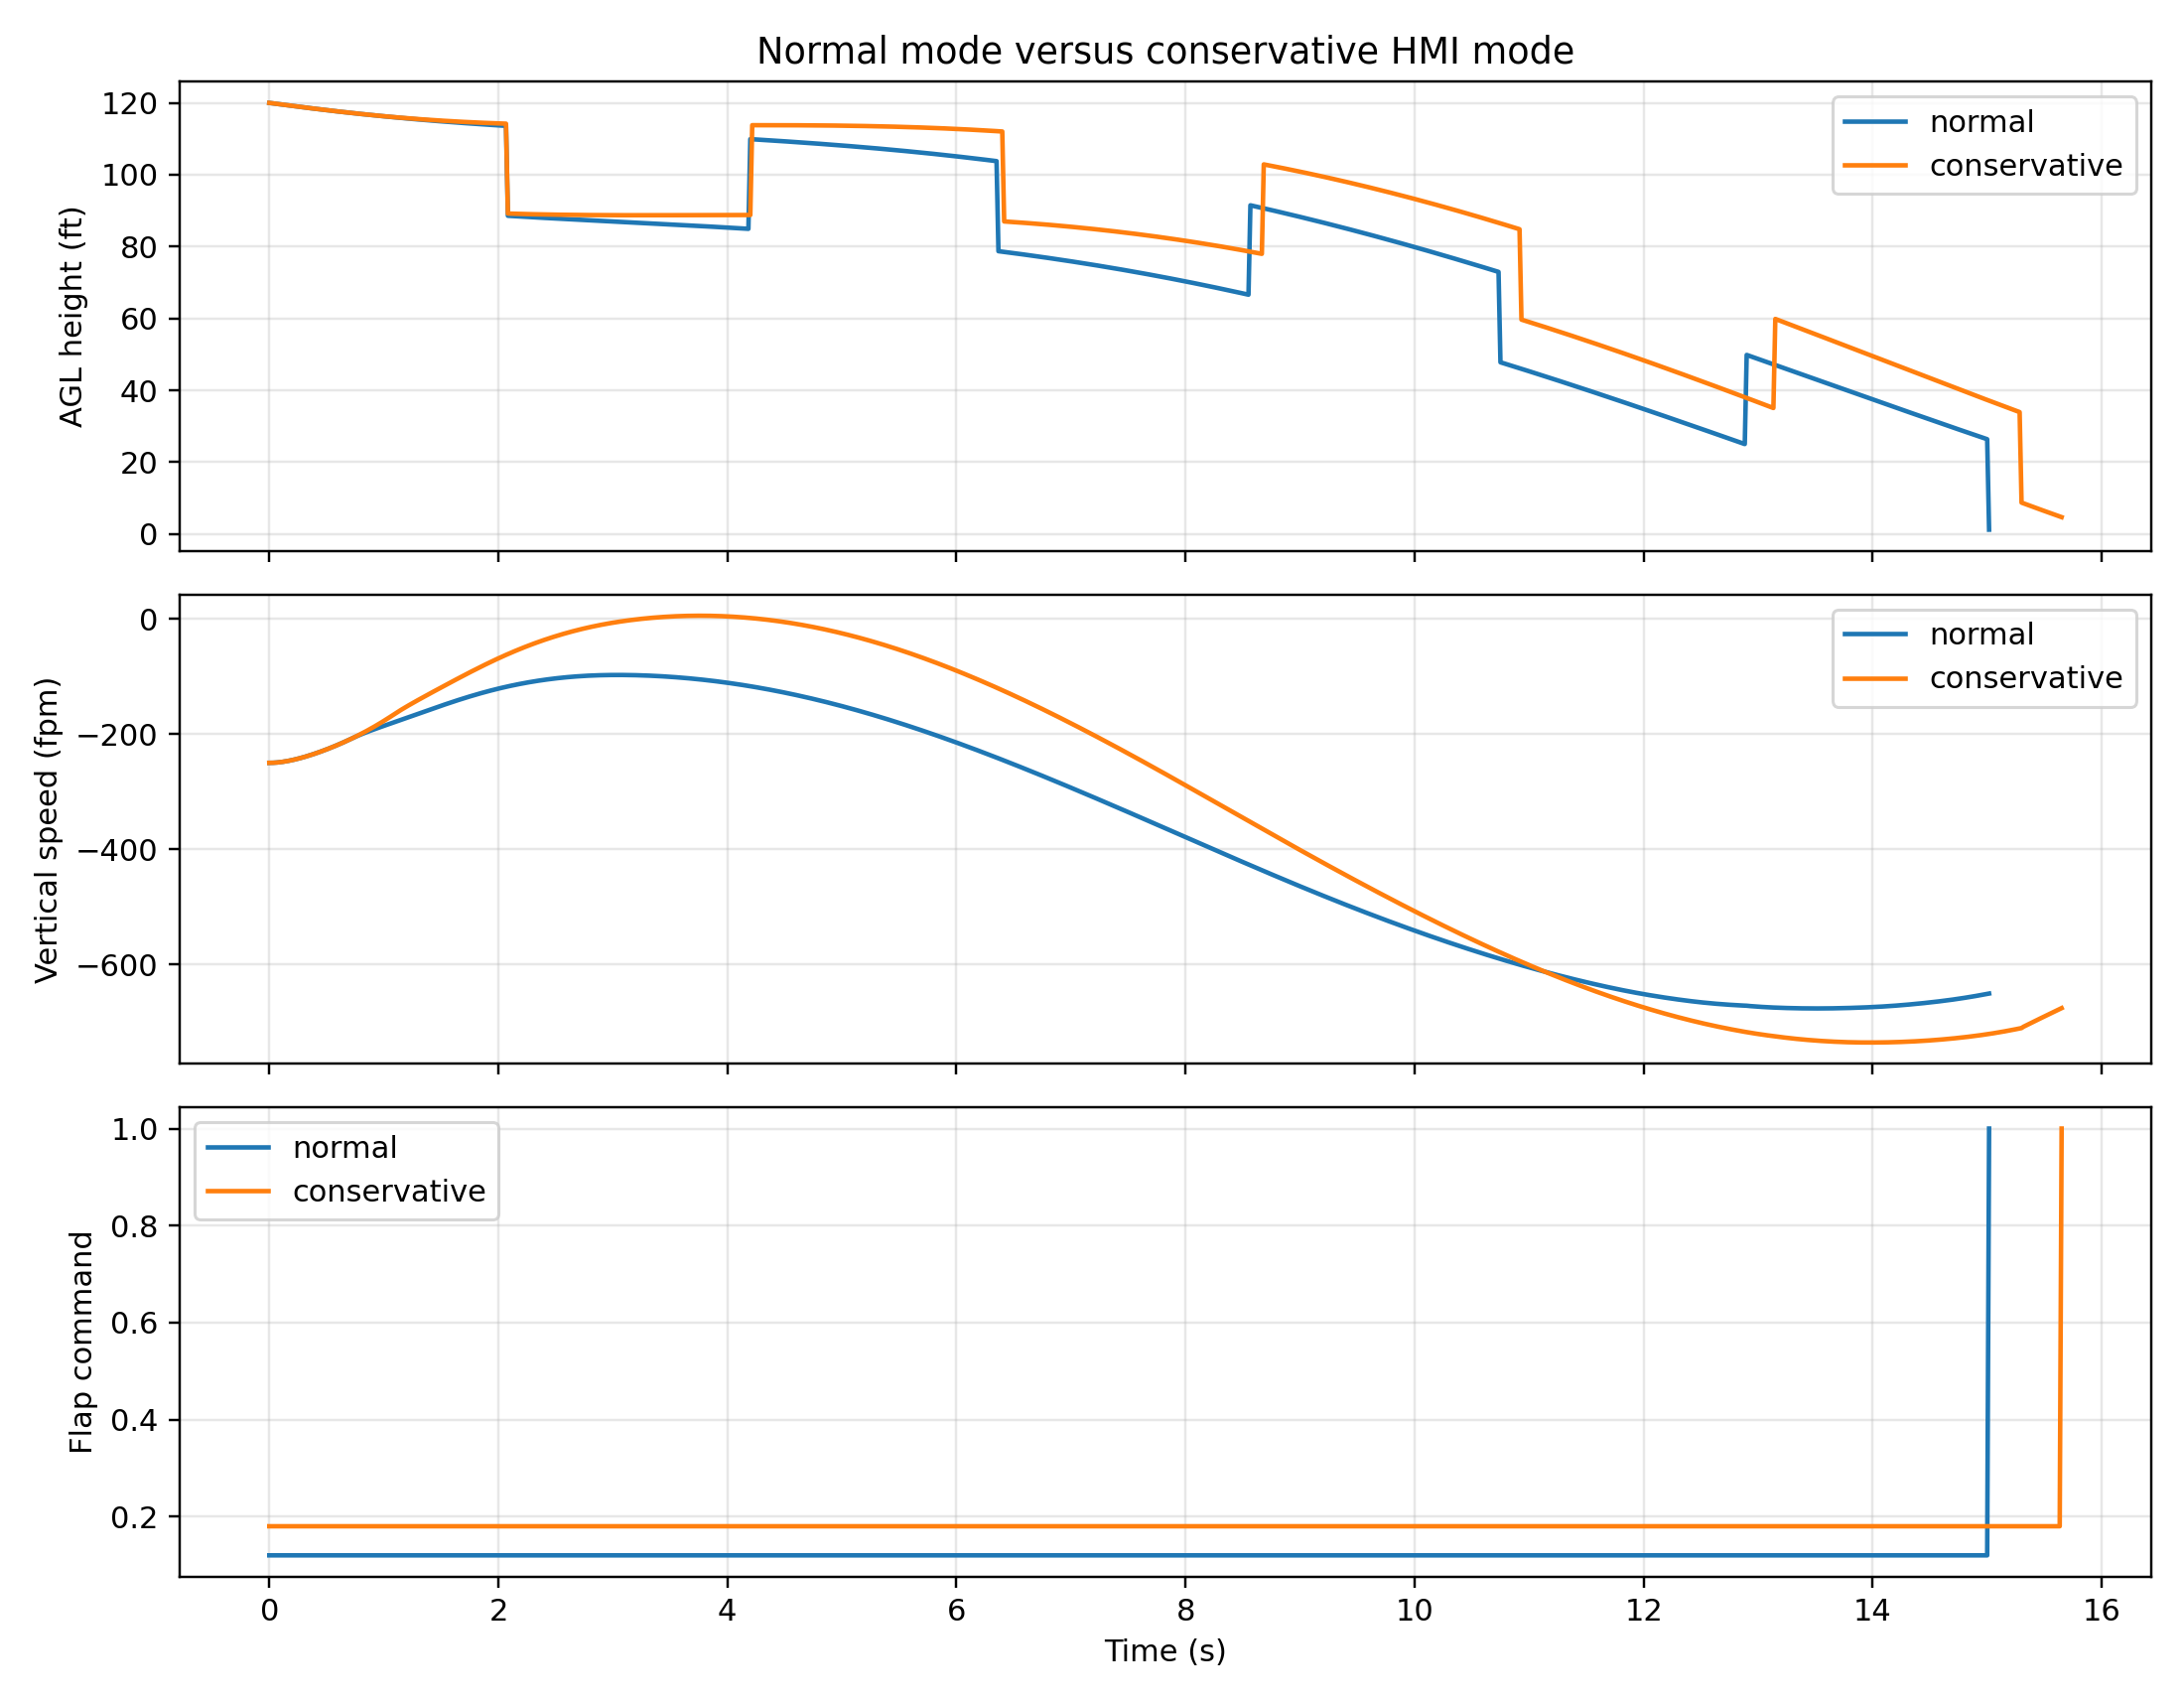
\includegraphics[width=5.19in,height=0.66\textheight,keepaspectratio]{images/image17.png}
\caption{正常模式与保守模式下着陆响应对比}
\label{fig:6-2}
\end{figure}

约束控制层为人机交互强化的最后一道保障。当根据前文风险识别判定飞行器已逼近危险边界，或者操纵输入有可能致使姿态快速恶化之际，系统需要针对部分输入实施限幅、整形或者强制约束。举例而言，在近地阶段对副翼和方向舵的过大修正予以限制，以此防止横向姿态突变，当速度过低时提高油门下限，避免进入危险低速区，在下沉率严重超出限定值时，触发更强的拉平控制或者复飞保护。约束控制的目的并非完全接管操纵，而是在关键窗口防止系统进入不可恢复状态。所以可以看出，状态提示、操纵辅助、约束控制并非相互孤立的三项功能，而是依据风险程度逐级增强的统一策略。

\section{关键参数敏感性分析}

为了弄清楚究竟哪些参数对于着陆品质、交互强化效果有着最为显著的影响，在本研究当中，需要针对关键参数进行敏感性分析工作。结合前文所提及的模型、工况结果，本研究挑选出目标速度、下沉率阈值、拉平高度、跑道捕获距离、侧偏约束、滚转角约束等作为敏感性分析的具体对象。之所以选择这些参数，主要是因为它们在控制逻辑里属于关键边界条件，并且与交互提示、保护动作的触发时机直接相关联。

为了能深入去分析系统对于初始状态偏差的敏感程度，本文专门建立了速度 -
侧偏二维工况矩阵，其中初始速度分别选取64、68、72、76、80
kts，初始侧偏选取 -100、-50、0、50、100
ft，地形环境设定为阶跃地形，随后引入综合风险评分来展开分析。从图6 -
3所呈现的热力图结果能够看出，低速并且侧偏较大的这种组合风险是最高的。这也就意味着速度的保持、侧向的修正乃是HMI提示最为关键重要的方面。

\begin{figure}[H]
\centering
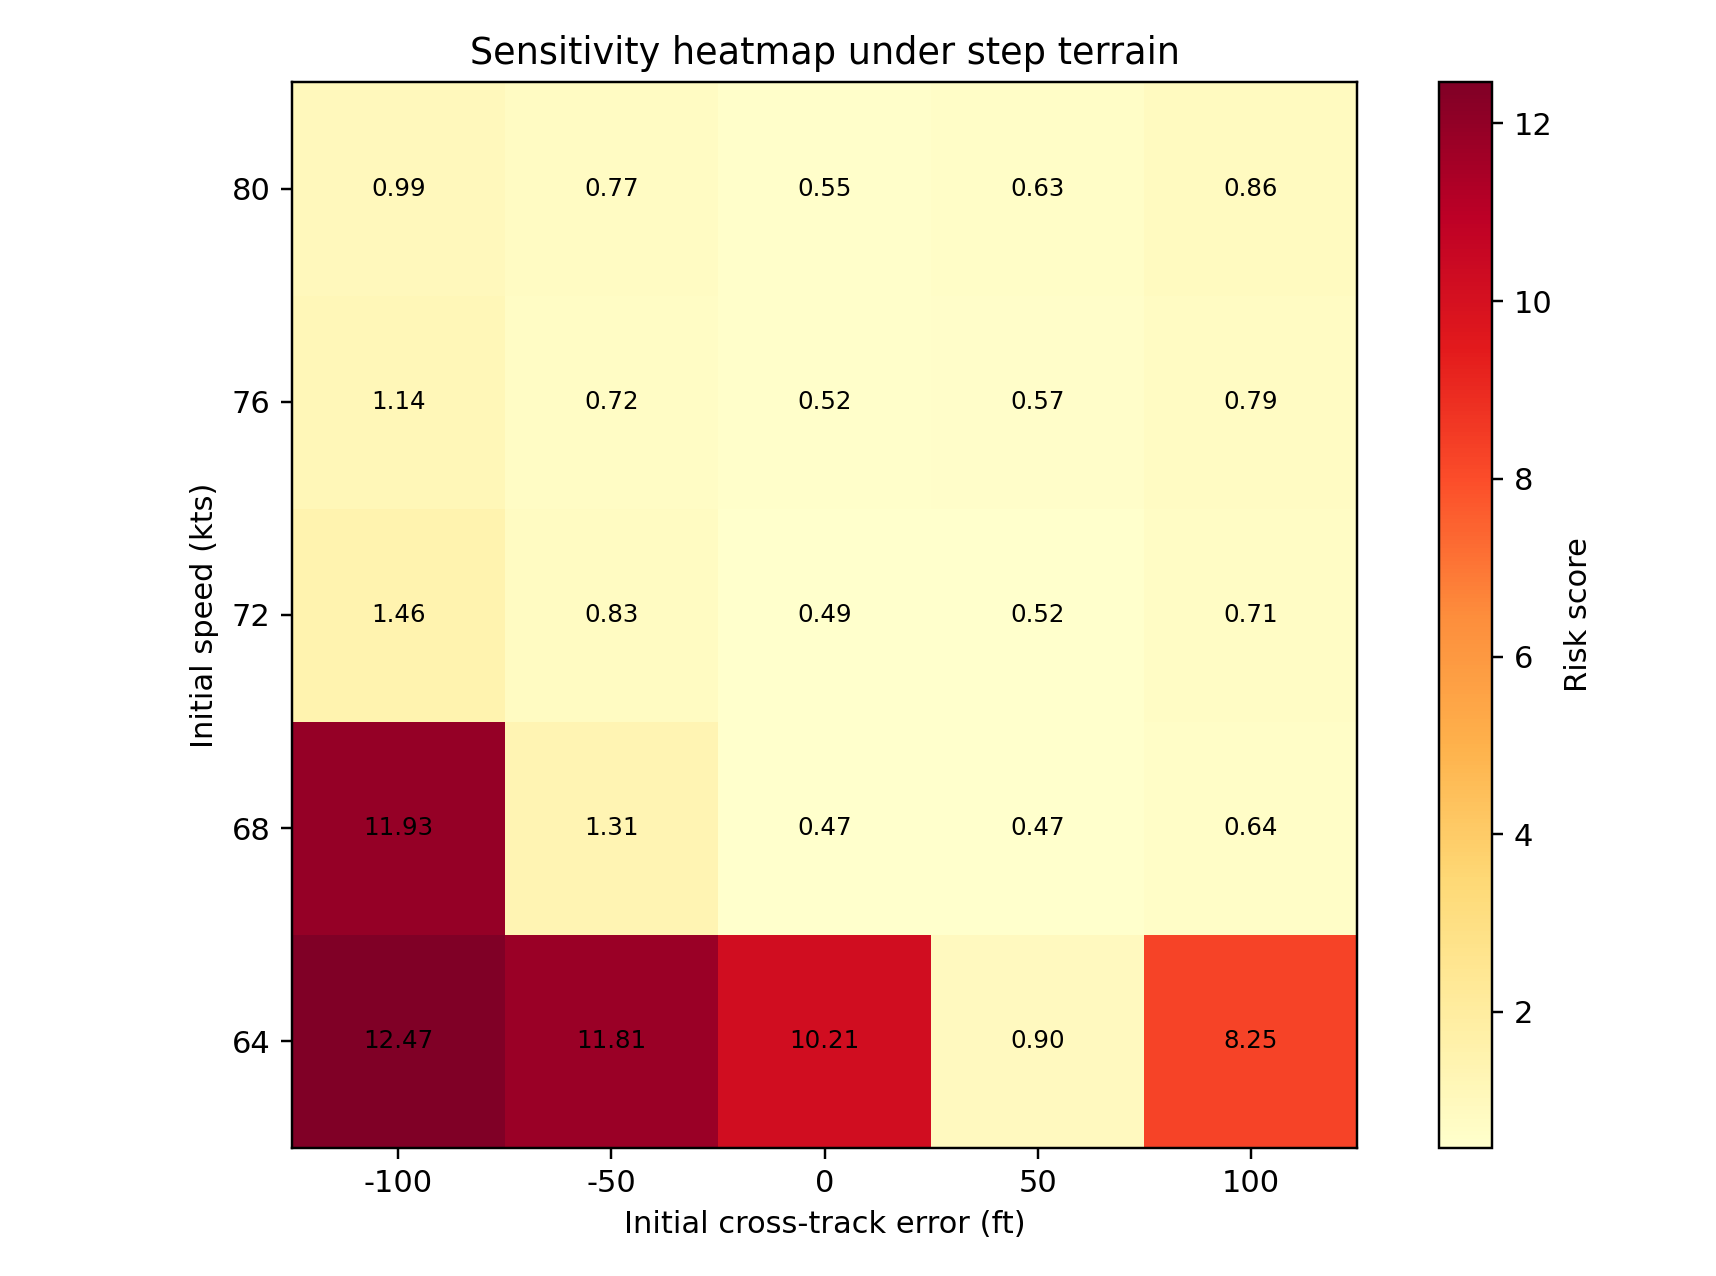
\includegraphics[width=5.43in,height=0.66\textheight,keepaspectratio]{images/image18.png}
\caption{初始速度与侧偏误差对风险评分的影响}
\label{fig:6-3}
\end{figure}

\section{改进建议与工程可实现性讨论}

借助敏感性分析能够发觉，目标速度、下沉率阈值、拉平高度对纵向品质造成的影响最为显著，而侧偏量和滚转角约束对横向稳定、跑道对准所产生的影响更为突出。这表明后续系统优化不可单纯平均地对所有参数予以调整，而应当优先围绕具备高敏感性的参数展开。喻小康在无人机概念设计与分析工具开发研究当中指出，参数化分析工具的价值体现在能够迅速识别影响系统性能的关键变量，进而提高方案迭代效率。所以，本文把敏感性分析当作连接仿真结果与工程优化的关键环节，用以给下一步参数调整、交互策略改进提供参考。

根据前文工况分析、敏感性分析的结果，本文认为针对人机交互强化的系统优化能够从四个方面着手进行。其一，对告警逻辑予以优化。需要进一步提高告警分级的针对性、可解释性，避免因提示过多而造成信息干扰，同时也要避免提示过晚进而失去干预价值。其二，优化状态显示方式。要突出离地高度、下沉率、速度、侧偏量等核心状态，以便让操纵者在末段能够迅速抓住重点，而非被大量辅助信息分散注意力。其三，优化操纵辅助策略。建议在不同的着陆阶段设置不一样的辅助优先级，比如在进近阶段优先给出轨迹与对准提示，在拉平阶段优先给出下沉率和俯仰控制提示，在接地区域优先给出稳定接地与方向保持提示。其四，优化约束控制边界。对于像拉平高度、速度下限、横向约束阈值这类高敏感参数，应当结合工况特征进行分阶段调整，而非采用固定不变的全程阈值。

为了验证约束保护策略的有效性，在本文中特意设置了大侧偏（260
ft）、大航向误差（35
deg）这样的极端工况。从图~\ref{fig:6-4}所呈现出的仿真结果能够看出，系统具备识别偏差越界的能力，并且会触发复飞保护，以此避免在不满足安全条件时还继续接地。这也就验证了约束保护层设计是很有必要的。

\begin{figure}[H]
\centering
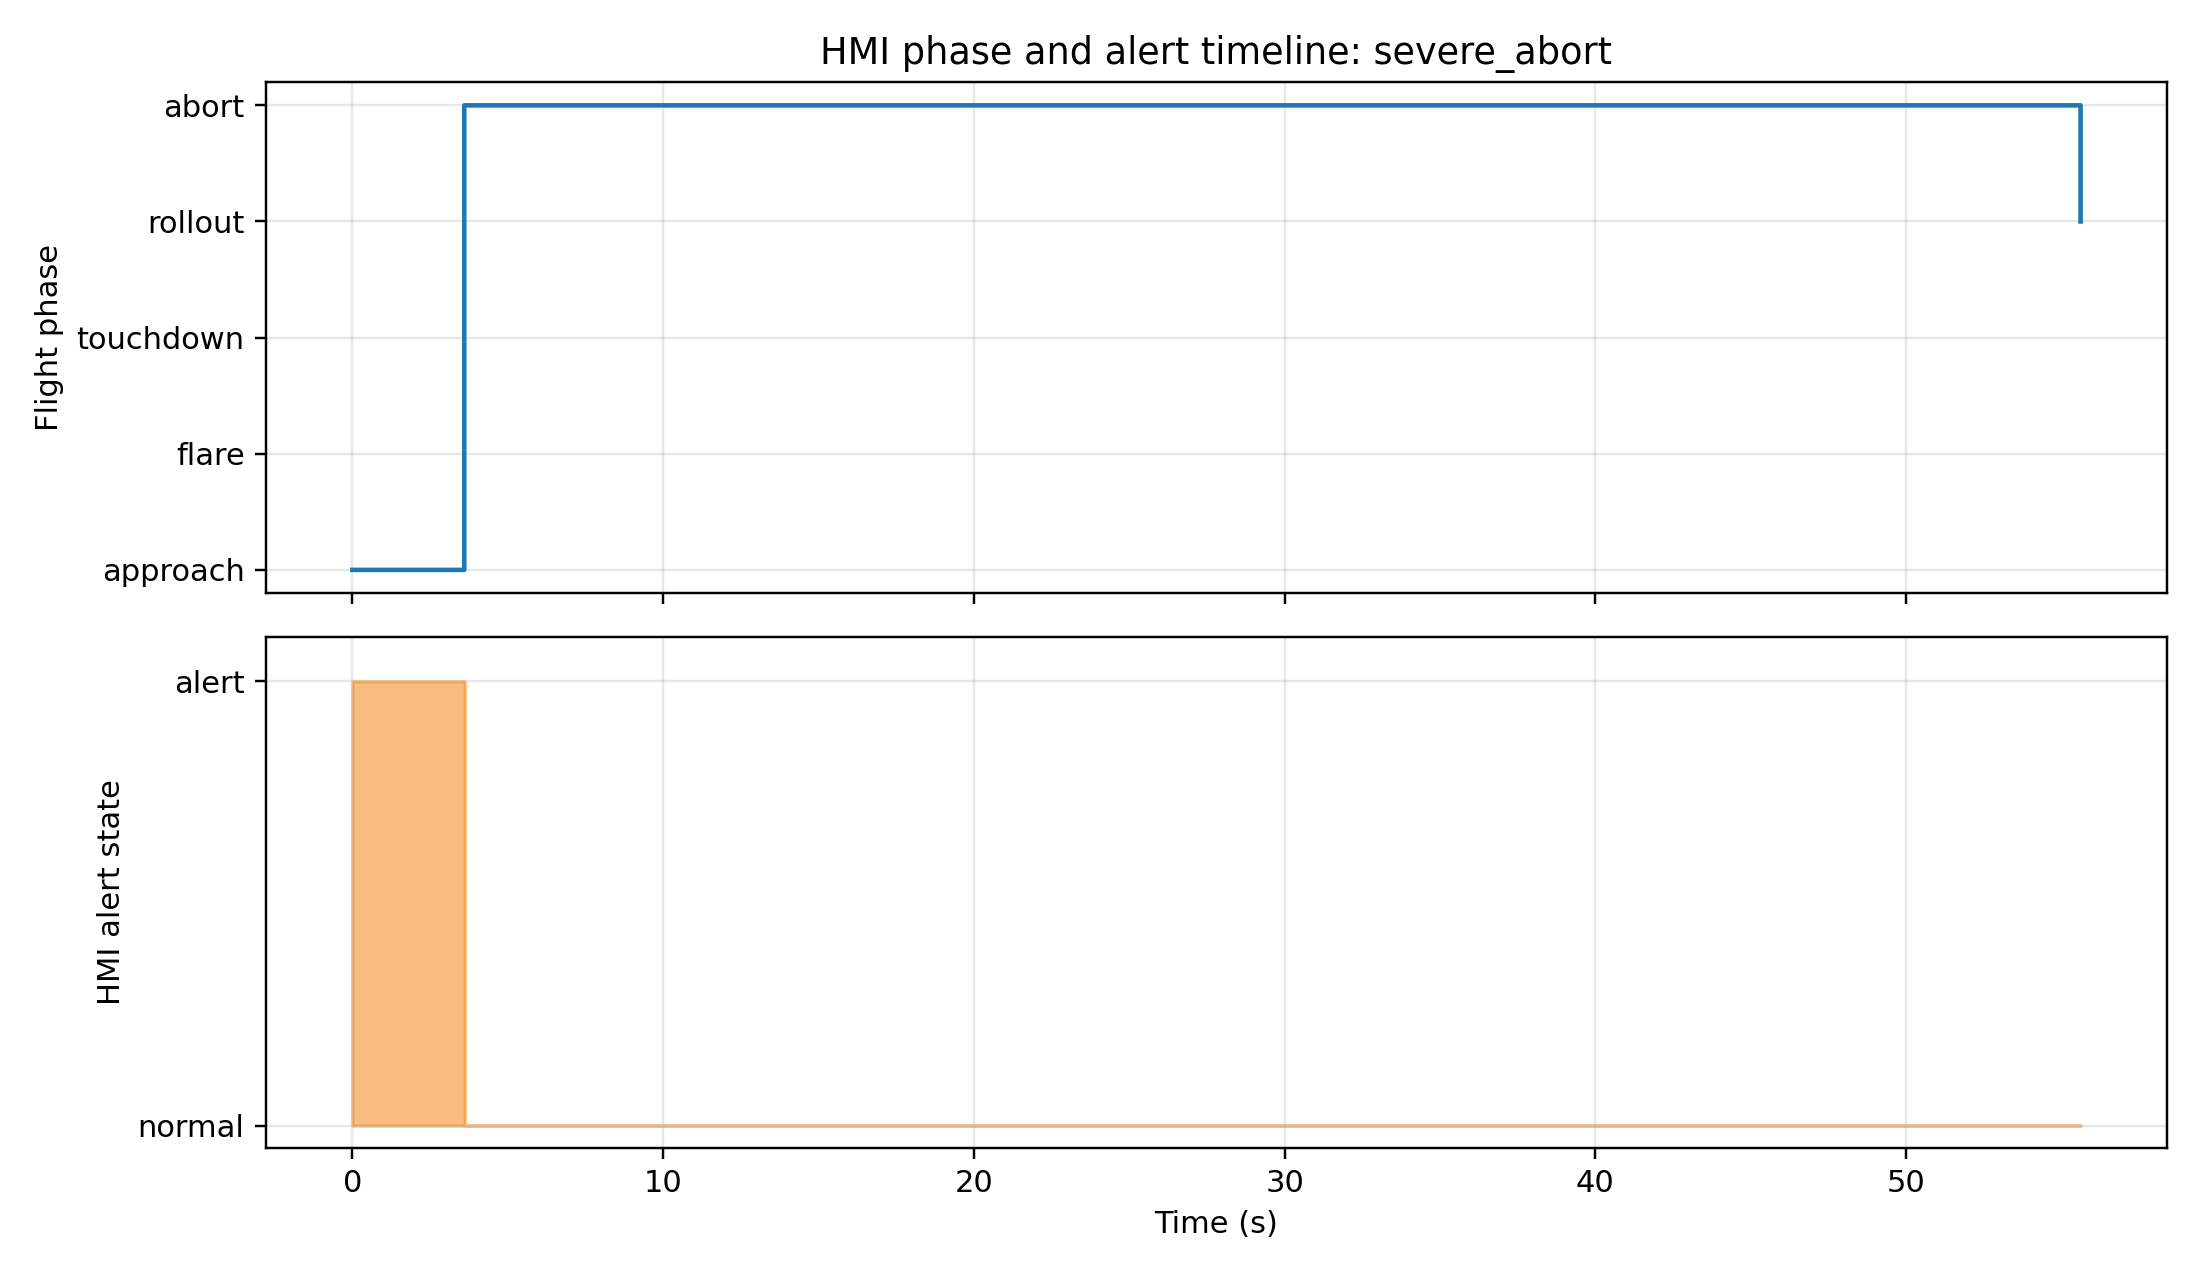
\includegraphics[width=0.92\linewidth,height=0.66\textheight,keepaspectratio]{images/image19.png}
\caption{极端偏差工况下复飞保护触发过程}
\label{fig:6-4}
\end{figure}

从工程能够实现的角度来看，本文所提出的人机交互强化策略具备良好的落地基础。第一，像速度、高度、姿态、侧偏量这些所需的关键状态量，都能够借助现有的飞控系统、导航感知系统来获取，无需额外建立太过复杂的硬件模式。第二，告警分级、状态提示、操纵辅助，本质上属于软件层的逻辑优化，可以通过飞控显示界面或者地面站界面来达成，开发成本相对而言比较低。第三，约束控制和复飞保护虽说对控制逻辑有较高要求，但在已有分阶段控制的基础上增添边界判断模块便能够实现，不需要重新建立一整套控制系统。所以，本文提出的优化策略既有理论分析的意义，也拥有一定的工程应用前景。

人机交互强化所具有的价值，并非在于替代飞行控制本身这一方面，而是在于借助``提前识别---及时提示---适度辅助---必要约束''此种方式，提高固定翼飞行器于复杂工况下的着陆稳定性、安全性。
